\section{Pregunta N$^{\circ}$1\qquad Andre Gilmer Santos Felix}

\begin{frame}
    \begin{enumerate}\setcounter{enumi}{0}
        \item

              Calcule la curvatura de la gráfica del polinomio de
              $B^{3}_{5}$.
    \end{enumerate}

    \begin{solution}
        La gráfica de una función $y=f\left(x\right)$ es un caso
        especial de una curva parametrizada, de la forma
        \begin{equation*}
            \begin{cases}
                x & =t               \\
                y & =f\left(t\right)
            \end{cases}
        \end{equation*}
        la curvatura viene dada por
        \begin{equation*}
            \kappa=
            \dfrac{
                y^{\prime\prime}
            }{
                {\left(1+{y^{\prime}}^{2}\right)}^{\frac{3}{2}}
            }.
        \end{equation*}

        \begin{figure}[ht!]
            \centering
            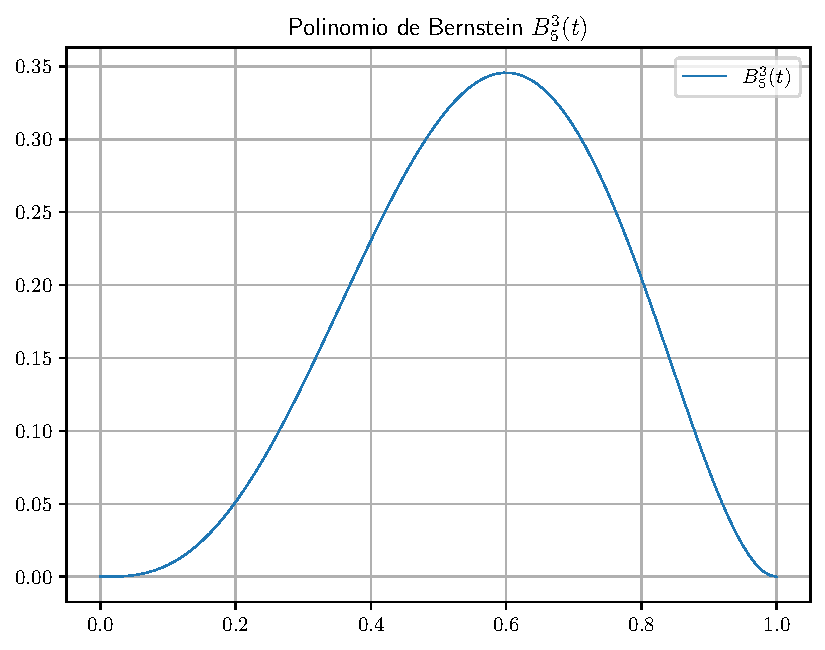
\includegraphics[width=.4\paperwidth]{p1}
        \end{figure}
    \end{solution}
\end{frame}

\begin{frame}
    \begin{solution}
       Los polinomios de Bernstein $B_{n}^{i}(t)$ se definen para $t$ en el intervalo $[0, 1]$ y se calculan de la siguiente manera:

\[B_{n}^{i}(t) = \binom{n}{i} \cdot t^i \cdot (1 - t)^{n - i}\]

Por ejemplo, para calcular $B_{5}^{3}(t)$ con $n = 5$ e $i = 3$, sustituyes estos valores en la fórmula:

\[B_{5}^{3}(t) = \binom{5}{3} \cdot t^3 \cdot (1 - t)^{5 - 3}\]

Calculamos el coeficiente binomial:

\[\binom{5}{3} = \frac{5!}{3!(5-3)!} = \frac{5 \cdot 4 \cdot 3!}{3! \cdot 2!} = \frac{5 \cdot 4}{2 \cdot 1} = 10\]

Luego, obtenemos:

\[B_{5}^{3}(t) = 10 \cdot t^3 \cdot (1 - t)^2\]

Esta es la expresión para el polinomio de Bernstein $B_{5}^{3}(t)$ específico.
 .
    \end{solution}
\end{frame}